%!TEX TS-program = xelatex
% !TeX spellcheck = en_GB 
\documentclass[11pt]{friggeri-cv}

\begin{document}
  \header{Gessica Trivelli}{Midwife}
  % In the aside, each new line forces a line break
  \begin{aside}
    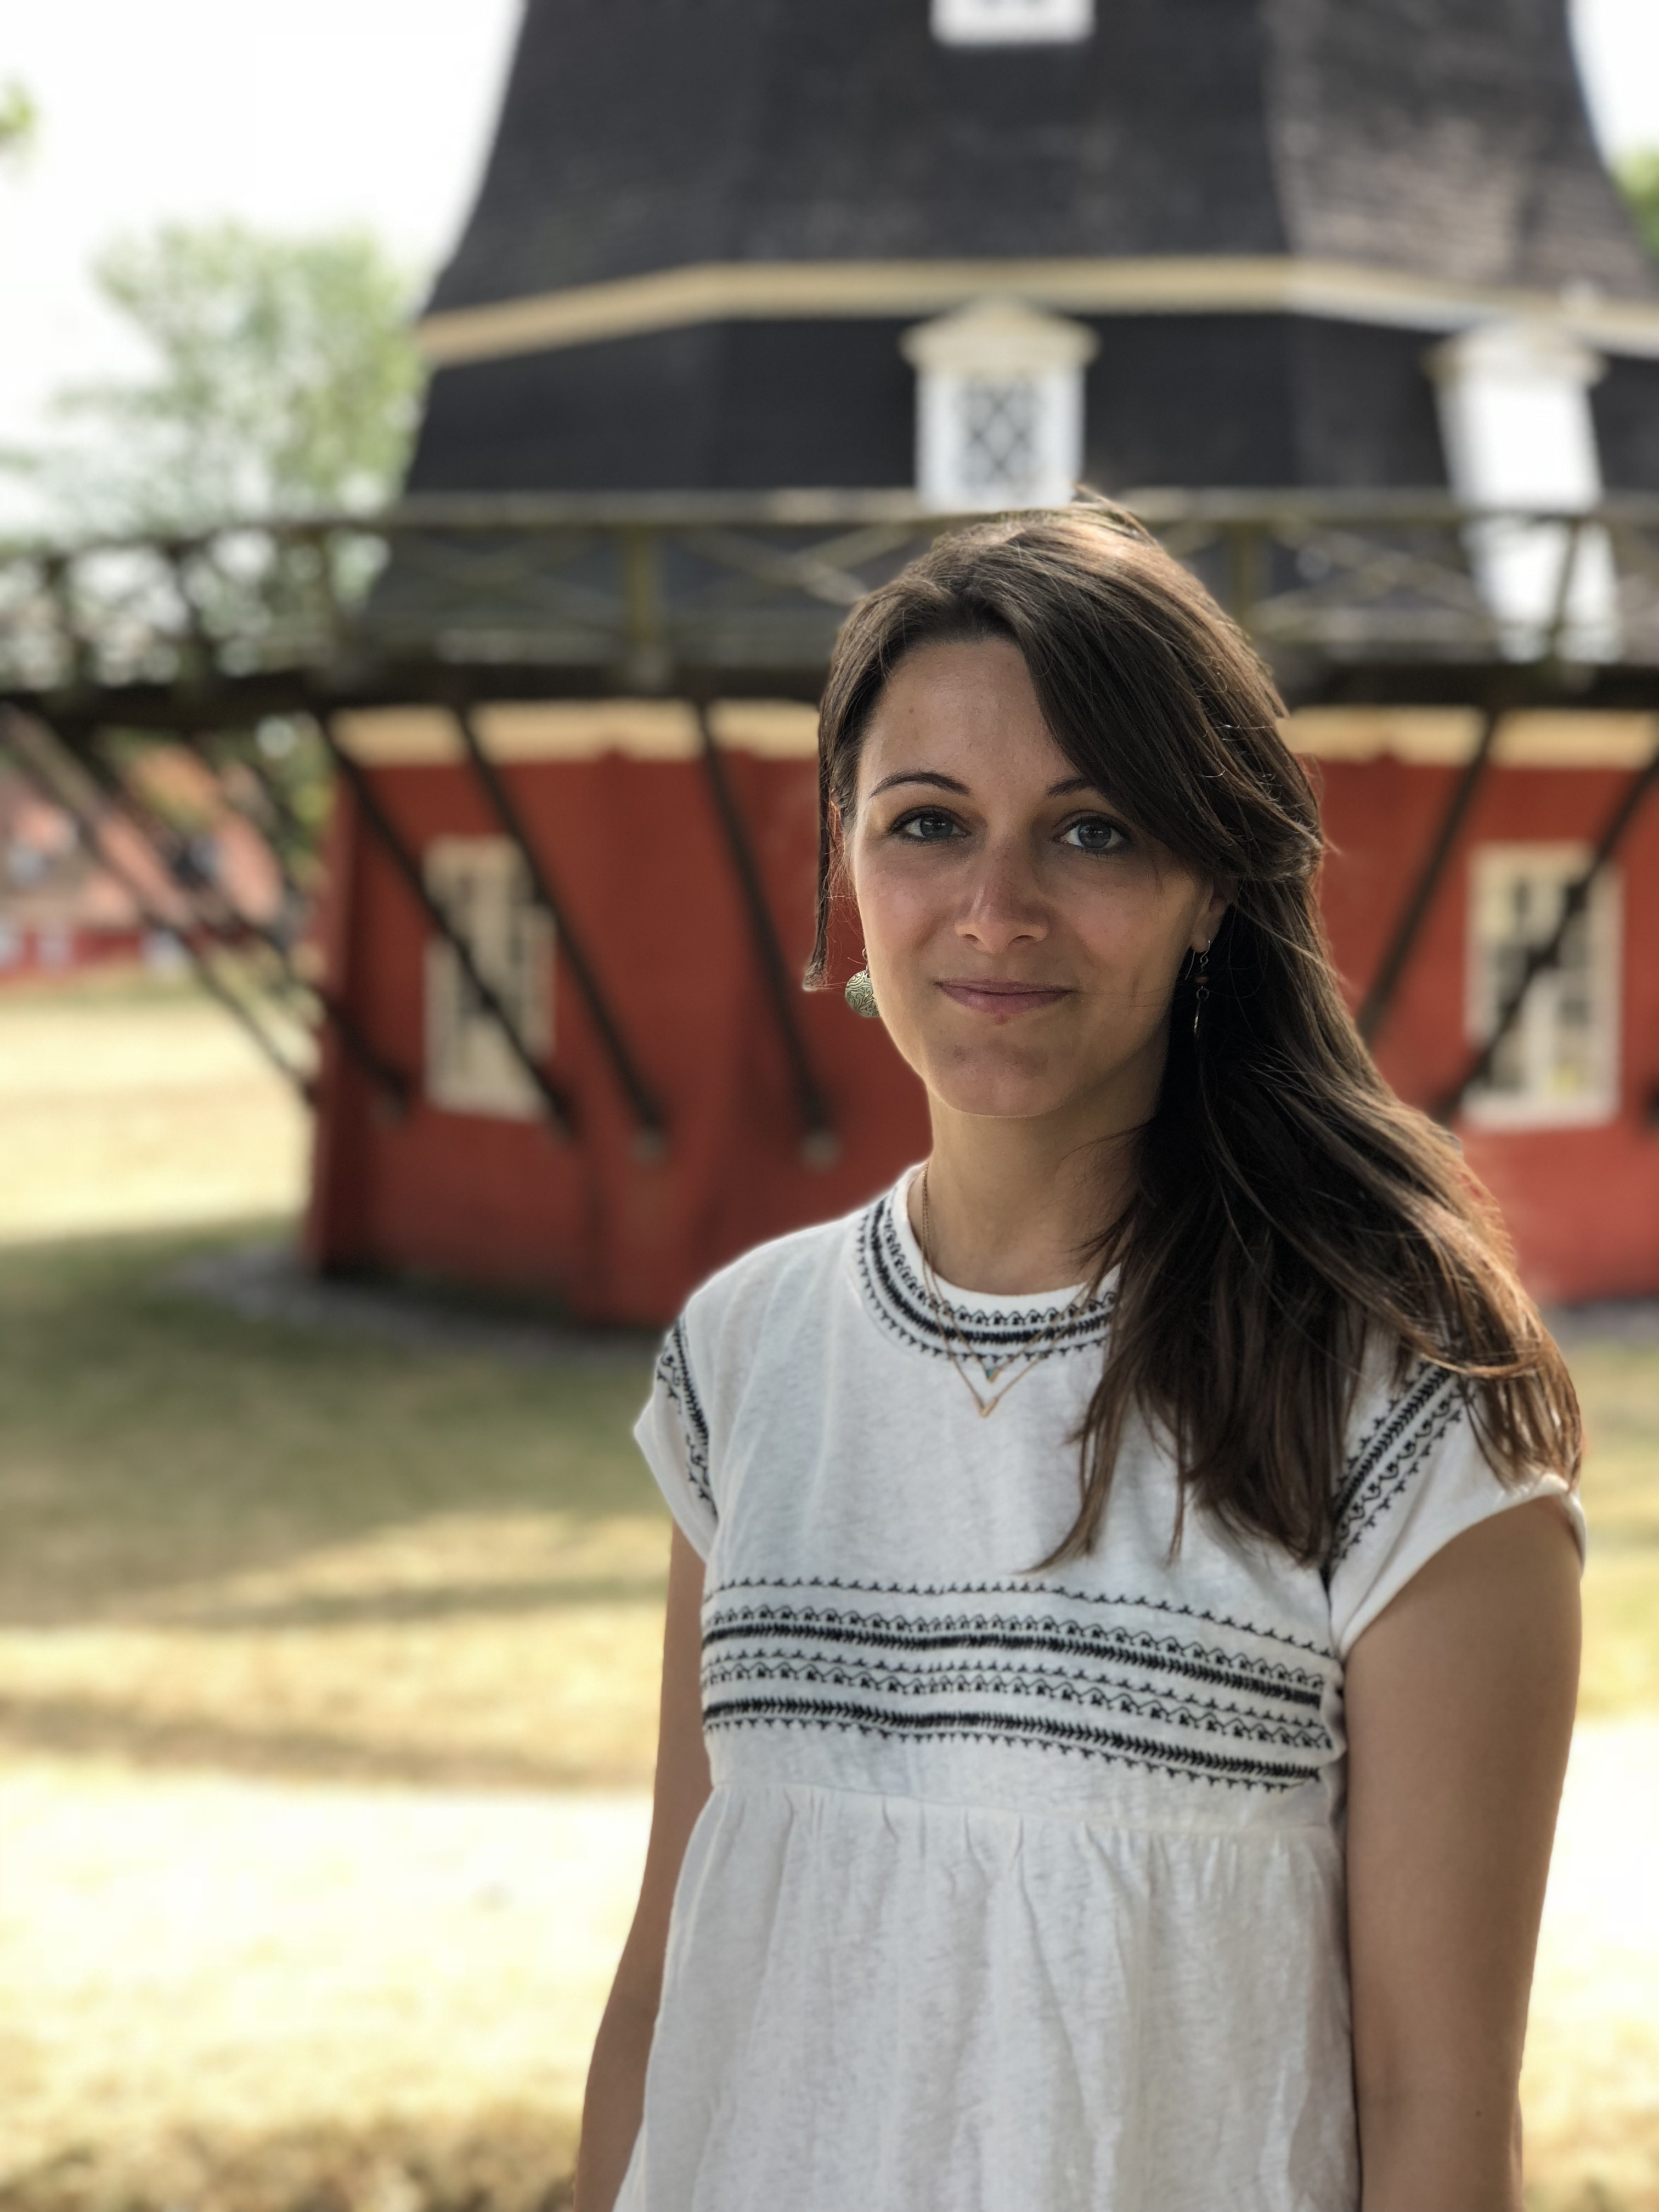
\includegraphics[width=0.95\columnwidth]{img/IMG_2838}
    \section{Skype}\footnotesize{
    gessica.trivelli@gmail.com}
    \section{Mail}\footnotesize{
    \href{mailto:gessica.trivelli@gmail.com}{gessica.trivelli@gmail.com}}
    \section{Personal Info}\footnotesize{
    \textbf{Nationality}: Italian
    \textbf{Birthday}: 14/04/1991}
  \end{aside}

\vspace{-10pt}
\section{Education}
\begin{entrylist}
  \entry
  {2017 - 2018}
  {Postgraduate Specialization in Midwifery [\small EQF 7]}
  {\\Scuola Elementale di Arte Ostetrica, Florence}
  {50 ECM Specialization Course - 194 hours - on the following topic: 
  \emph{Pelvic floor's health in female cycle: education, prevention 
  re-education and treatment of perineal dysfunction using a midwifery-led 
  approach.}\\
  Thesis title: \emph{Pelvic Organ Prolapse: beyond the surgery}.\\}
  
  \entry
  {2014 - 2017}
  {Master's Degree in Nursing and Midwifery [\small EQF 7]}
  {\\Tor Vergata University of Rome}
  {First Class with Honors. \\Internship - thesis at \textit{"Istituto 
  Superiore di Sanita'"} on the following topic: \textit{Health knowledge, 
  attitudes and practice of midwifery students, pregnant women and midwives on 
  umbilical cord clamping and cord blood stem cells transplantation.}\\}
  
  \entry
  {2010 - 2014}
  {Bachelor's Degree in Midwifery [\small EQF 6]}
  {\\Tor Vergata University of Rome}
  {First class with honors.\\
  Internship in Rome in several hospitals: \textit{Policlinico Tor Vergata}, 
  \textit{Azienza Ospedaliera San Giovanni Addolorata}, \textit{Ospedale 
  Fatebenefratelli San Giovanni Calibita} and \textit{Policlinico Casilino}.\\
  Thesis title: \textit{Survey on Women's Positions during Labour and Delivery: 
  Evaluation of Maternal and Foetal Outcomes.}\\}
  
  \entry
  {2005-2010}
  {Scientific Diploma [\small EQF 4]}
  {\\Scientific High School "A. Gentili", Sarnano (MC)}
  {}
\end{entrylist}

\vspace{-20pt}
\section{Experience}
\begin{entrylist}
  \entry
    {2019 - \\now}
    {Midwife}
    {\\Helios Klinik in Titisee-Neustadt, Germany}
    {Delivery suite.}
  
  \entry
    {2017 - \\2018/11}
    {Midwife}
    {\\Coombe Women and Infants University Hospital of Dublin, Ireland}
    {Outpatient Department (Midwifery and Gynaecology Clinic)\\
     Midwifery and Advanced Care.\\
     Emergency Department.}
\end{entrylist}
\newpage

\begin{aside}
  \section{IT Skills}
  \textbf{Office}
\includegraphics[scale=0.40]{img/5stars.png}
  \textbf{Epi-Info}
\includegraphics[scale=0.40]{img/3stars.png}
  \textbf{Pubmed}
\includegraphics[scale=0.40]{img/5stars.png}
  ~
  \section{Relational Skills}\footnotesize{
  Women-centred care, promoting information and free decision making, through 
  skills such as counselling, empathy and active listening}.
  ~
  \section{Technical Skills}\footnotesize{
  Problem solving
  ~
  Use of brand new and innovative didactic models
  ~
  Education in the adulthood
  ~
  Planning, implementation and evaluation of clinical, organizational and 
  pedagogical topics
  ~
  Quantitative and qualitative research in clinical, organizational and 
  pedagogical fields
  ~
  Evaluation of care services (e.g. quality, pertinence, safety and cheapness)}
\end{aside}

\vspace{-15pt}
\section{Certifications}
\begin{entrylist}
  \entry
    {2018}
    {BLS provider - American Heart Association}
    {\\Center for Midwifery Education, Dublin - Irish Heart Foundation}
    {\vspace{-10pt}}
  \entry
    {2018}
    {K2MS Perinatal Training Programme (PTP).}
    {\\K2MS, Dublin}
    {Fetal monitoring and maternity crisis management training}
  \entry
    {2018}
    {Breastfeeding Refresher Programme}
    {\\Center for Midwifery Education, Dublin}
    {\vspace{-10pt}}
  \entry
    {2018}
    {Diabetes in Pregnancy Update}
    {\\Center for Midwifery Education, Dublin}
    {\vspace{-10pt}}
  \entry
    {2018}
    {Preceptorship Programme for Midwives and Nurses}
    {\\Center for Midwifery Education, Dublin}
    {\vspace{-10pt}}
  \entry
    {2018}
    {Water Immersion for Labour and Birth}
    {\\Center for Midwifery Education, Dublin}
    {\vspace{-10pt}}
  \entry
    {2017}
    {Haemovigilance and Infection Control}
    {\\Center for Midwifery Education, Dublin}
    {\vspace{-10pt}}
  \entry
    {2016}
    {Emergencies During Delivery}
    {\\CreAttivaMente Ostetriche, Rome}
    {16 hours course, using medical mannequin.}
  \entry
    {2015}
    {Advanced skills to support breastfeeding}
    {\\CreAttivaMente Ostetriche, Rome}
    {16 hours course.}
  \entry
    {2014}
    {Breastfeeding: councelling practical course, OMS/UNICEF model}
    {\\Tor Vergata Universiy of Rome}
    {40 hours course.}
\end{entrylist}

\vspace{-15pt}
\section{Languages}
\begin{table*}[!h]
  \centering
  \renewcommand{\arraystretch}{1.45}
  \begin{tabular}{ p{3cm} p{3cm} p{3cm} p{3cm} }
    \hline
      & \textbf{Written}  
      & \textbf{Spoken} 
      & \textbf{Listening} \\ 
    \hline
    \textbf{Italian:}   
      & \multicolumn{3}{c}{Mother-tongue} \\
    \textbf{English:}
      & C1 
      & C1 
      & C1 \\ 
    \textbf{German:} 
      & B2 
      & B2 
      & B2 \\ 
    \textbf{French:} 
      & A1 
      & A1 
      & A2 \\
    \hline
  \end{tabular}
\end{table*}

\newpage
\section{Honours \& Awards}
\begin{entrylist}
  \entry
    {2016}
    {Tutor Scholarship}
    {\\Tor Vergata University of Rome}
    {250 ore}
  \entry
    {2013}
    {Cooperation Scholarship}
    {\\Tor Vergata University of Rome}
    {150 ore}
\end{entrylist}

\section{Other informations}
\begin{itemize}
  \item[--] Subscribed to the \textit{Collegio Ostetriche of Rome} since 
  February 2015 (n. 2640).
  \item[--] Subscribed to the \emph{Land Baden-W{\"u}rttenberg 
    Regierungspr{\"a}sidium Stuttgart} since July 2019.
\end{itemize}


\vspace{3.5cm}
\begin{flushleft}
  \large\emph{Rome, August 23rd 2019}
\end{flushleft}
\begin{flushright}
  \large\emph{Gessica Trivelli}
\end{flushright}

\end{document}
